%This is a very basic  BE PROJECT PRELIMINARY template.

%############################################# 
%#########Author :  PROJECT###########
%#########COMPUTER ENGINEERING############


\documentclass[oneside,a4paper,12pt]{report}
%\usepackage{showframe}
%\hoffset = 8.9436619718309859154929577464789pt
%\voffset = 13.028169014084507042253521126761pt

\fancypagestyle{plain}{%
  \fancyhf{}
  \fancyfoot[CE]{College_Name, Department of Computer Engineering 2015}
  \fancyfoot[RE]{\thepage}
}
\pagestyle{fancy}
\fancyhead{}
\renewcommand{\headrulewidth}{0pt}
\footskip = 0.625in
\cfoot{}
\rfoot{}
\usepackage{amsmath}
\usepackage[]{hyperref}
\usepackage{tikz}
\usetikzlibrary{arrows,shapes,snakes,automata,backgrounds,petri}

\usepackage{tabularx}
\usepackage[euler]{textgreek}

%\usepackage[nottoc,notlot,notlof,numbib]{tocbibind}
\usepackage[titletoc]{appendix}
\usepackage{titletoc}
\renewcommand{\appendixname}{Annexure}
\renewcommand{\bibname}{References}

\setcounter{secnumdepth}{5}

\usepackage{float}
\usepackage{subcaption}
\usepackage{multirow}

\usepackage[ruled,vlined]{algorithm2e}

\begin{document}

\setlength{\parindent}{0mm}
\begin{center}
{\bfseries A PRELIMINARY PROJECT REPORT ON  \\}
 \vspace*{1\baselineskip}
{\bfseries INPAINTING OF DEGRADED DOCUMENT IMAGE USING 
DEEP NEURAL NETWORK \\}
 \vspace*{1\baselineskip}
{\fontsize{12}{12} \selectfont SUBMITTED TO SAVITRIBAI PHULE PUNE UNIVERSITY, PUNE IN PARTIAL FULFILMENT OF THE REQUIREMENTS FOR THE AWARD OF THE DEGREE \\ 
OF
\vspace*{1\baselineskip}}

{\bfseries \fontsize{16}{12} \selectfont BACHELOR OF ENGINEERING (COMPUTER ENGINEERING) \\
\vspace*{1\baselineskip}} 
{\bfseries \fontsize{12}{12} \selectfont SUBMITTED BY \\ 
\vspace*{1\baselineskip}} 
 Sayali Mahajan\hspace{25 mm} Exam No: B150134308 \\ 
 Kranti Pawar \hspace{25 mm}  Exam No: B150134344 \\  
 Sonali Wagh  \hspace{25 mm}  Exam No: B150134347 \\
 Ankush Jadhav\hspace{25 mm}  Exam No: B150134333 \\
 Himanshu Shekhar\hspace{25 mm}  Exam No: B150134337 \\
\vspace*{2\baselineskip}

\includegraphics[width=100pt]{collegelogo.png} \\
{\bfseries \fontsize{16}{12} \selectfont DEPARTMENT OF COMPUTER ENGINEERING \\ 
 \vspace*{1\baselineskip}

K. K. Wagh Institute Of Engineering Education \& Research\\ 
}
 \vspace*{1\baselineskip}
{\bfseries \fontsize{12}{12} \selectfont 
Hirabai Haridas Vidyanagari, Amrutdham, Panchavati, Nashik-422003 
\vspace*{1\baselineskip}}
{\bfseries \fontsize{12}{12} \selectfont 
SAVITRIBAI PHULE PUNE UNIVERSITY\\
2018-19
}
\end{center}

\newpage





{\bfseries \fontsize{12}{12} \selectfont \centerline{SAVITRIBAI PHULE PUNE UNIVERSITY }
}

{\bfseries \fontsize{12}{12} \selectfont \centerline{2018-19}
\vspace*{1\baselineskip}}

\begin{figure}[ht]
\centering

\includegraphics[width=100pt]{collegelogo.png}
\end{figure}

{\bfseries \fontsize{14}{12} \selectfont \centerline{K. K. Wagh Institute Of Engineering Education \& Research}
\vspace*{1\baselineskip}} 


{\bfseries \fontsize{14}{12} \selectfont \centerline{CERTIFICATE} 
} 

\centerline{This is to certify that the Project Entitled}
\vspace*{1\baselineskip} 


{\bfseries \fontsize{12}{12} \selectfont \centerline{"BE PROJECT TITLE"}
\vspace*{1\baselineskip}}

\centerline{Submitted by}
\vspace*{1\baselineskip} 
\centerline{Sayali Mahajan  \hspace{25 mm} Exam No:B150134308 } 
\centerline{Kranti Pawar \hspace{25 mm} Exam No:B150134344  } 
\centerline{Sonali Wagh \hspace{25 mm} Exam No:B150134347 }
\centerline{Ankush Jadhav \hspace{25 mm} Exam No:B150134333 }
\centerline{Himanshu Shekhar \hspace{25 mm} Exam No:B150134337 }
\vspace*{1\baselineskip} 
is a bonafide work carried out by Students under the supervision of Prof. Guide Name and it is approved for the partial fulfilment of the requirement of Savitribai Phule Pune University, for the award of  Bachelor of Engineering (Computer Engineering).\\

\bgroup
\def\arraystretch{0.7}
\begin{tabular}{c c }
Prof. Guide Name &  \hspace{50 mm} Prof. HOD Name \\								
Internal Guide   &  \hspace{50 mm} H.O.D \\
Dept. of Computer Engg.  &	\hspace{50 mm}Dept. of Computer Engg.  \\
\end{tabular}
%}
\vspace*{0.1\baselineskip} 
\begin{center}
%\fontsize{12}{18}\selectfont 
{
Dr. K. N. Nandurkar \\
Principal\\
}
\end{center}
Place: Nashik\\
Date: 
%}



\newpage


\setcounter{page}{0}
\frontmatter
\cfoot{KKWIEER, Department of Computer Engineering 2018-19}
\rfoot{\thepage}
\pagenumbering{Roman}


		

{  \newpage {\bfseries \fontsize{14}{12} \selectfont \centerline{ACKNOWLEDGEMENT} 
\vspace*{2\baselineskip}} \setlength{\parindent}{11mm} }
{ \setlength{\parindent}{0mm} }
\textit{It gives us great pleasure in presenting the preliminary project report 
on {\bfseries \fontsize{12}{12} \selectfont `INPAINTING OF DEGRADED DOCUMENT IMAGE USING 
DEEP NEURAL NETWORK'}.}
\vspace*{1.5\baselineskip}

 \textit{We would like to take this opportunity to thank our internal guide
 \textbf{Prof. Smita Patil} for giving us all the help and guidance we needed. We are
 really grateful to them for their kind support. Their valuable suggestions were very helpful.} \vspace*{1.5\baselineskip}

 \textit{We are also grateful to \textbf{Dr. S.S.Sane}, Head of Computer
 Engineering Department, CollegeName for his indispensable
 support, suggestions.}
\vspace*{1.5\baselineskip}

\textit{In the end our special thanks to \textbf{Prof. Anand Kolapkar and Prof. Suruchi Malao} for
providing various resources such as  laboratory with all needed software platforms,
continuous Internet connection, for our Project.}
\vspace*{3\baselineskip} \\
\begin{tabular}{p{8.2cm}c}
&Sayali Mahajan\\
&Kranti Pawar\\
&Sonali Wagh\\
&Ankush Jadhav\\
&Himanshu Shekhar\\
&(B.E. Computer Engg.)
%}
\end{tabular}

{  \newpage {\bfseries \fontsize{14}{12} \selectfont \centerline{ABSTRACT} 
\vspace*{2\baselineskip}} \setlength{\parindent}{11mm} }
{ \setlength{\parindent}{0mm} }
Document Images get degraded due to unbalance illumination spread over document including smearing of text, bleeding of ink to the other side of page, degradation of paper ink due to aging, manuscript characters from background side appear as noise on the
lead side and get blend with the lead side characters etc. Binarization is used to recover text from degraded document
images. Recovering text from degraded document images is a very difficult task due to inter or intra variation between background and foreground pixels.
Then an interpolation inpainting is performed to create the background estimationand foreground (text) estimation, that will be used as feature to train and test a su-pervised artificial neural network. We are going to perform Deep Neural Network (DNN) to learn about the text pixeland background pixels and define the edges of the text pixels


% \maketitle
\tableofcontents
\listoffigures 
\listoftables



\mainmatter



  \titleformat{\chapter}[display]
{\fontsize{16}{15}\filcenter}
{\vspace*{\fill}
 \bfseries\LARGE\MakeUppercase{\chaptertitlename}~\thechapter}
{1pc}
{\bfseries\LARGE\MakeUppercase}
[\thispagestyle{empty}\vspace*{\fill}\newpage]







\setlength{\parindent}{11mm}


			
\chapter{Introduction}
\section{Motivation}
There are different motivations for this project, all related to image processing and machine learning domain. The proposed application will be used in different archives where there is need for document preservation. \\
Our research is based on the Deep Neural Network and Convolutional Neural Network  which is one part of Artificial Network. It is going to have multiple hidden layer, each layer filtering multi-degradation of an image. At Every stage we are
\\ removing \& adding new layer to remove the degradation in the original image.

\section{Problem Definition And Objectives}
The goal of the document image binarization is to create a
perfect separation between text pixels and background pixels,
The binarization is a type of classification problem that segment the document image into two classes: 0 or 1.\\
Unfortunately, most of the historical document images suffer
from different types of degradation, such as bleed-through,
large stains, tears ink, blur. Figure (1) shows some examples
of degradation. Those multiple degradation make the process
of binarization a challenging task for researchers.
The good results of the binarization step are inescapable for
improving the quality of text recognition system and document
image analysis.
Our work here is mainly focused on the recovering the degraded part of the image or we can say the stained part. In some cases it can be entire image. The method exploit the benefit of the artificial network with an automatic extraction of features. This extraction is done with an inpainting phase in two way: one for erase the text pixels to get the background pattern , and the second one to erase the background pixels to get a text pattern.

\section{Project Scope and Limitation}
A good Software Requirement Specification(SRS) defines how an application will interact with system hardware, other programs and human users in a wide variety of real world situations. Parameters such as operating speed, response time, availability, portability, maintainability, footprint, security and speed of recovery from adverse events are evaluated.
Scope of our project deals with degraded region of the degraded document image. Unlike other applications available in the market
its scope is limited to only small research purposes. Basically our project is likely to help understand the working idea behind the Inpainting or Binarization of degraded document image with the help of Deep Learning.
As all the system has some limitation so does this. First of all
limitations based on the input images provided to the system.
Secondly the deep learning implementation on the system sometimes causes to change the pixel parts due to the unwanted filling operations.

\section{Methodologies of Problem Solving}
Our approach to solve the project is very basic i.e. Divide and Conquer. We have divided project into small stages as follows, taking image as input and covert it to its respective grey-scale and simultaneously applying Gaussian filter with varying sigma values. Module two do the Adaptive Threshold part i.e. applying
one of available algorithm for Binarization i.e. Otsu's, Sauvolas', etc. Third and fourth part is to apply morphology i.e. performing dilation and erosion operation respectively to get the text pixel class or background pixel class. Then our final module will train and test the same operations on the set of images so that our deep neural network can learn and predict the output image. 

\chapter{Literature Survey}
\begin{itemize}
\item Title: A Binarization Method for Degraded Document
Image using Artificial Neural Network and Interpolation Inpainting.\\
Author: Naouel Ouafek, Mohamed-Khireddine Kholladi\\
Description:The binarization of degraded document image is an
important phase in the document analysis to extract text from
the original image. For this purpose, we present a new multi-
stage approach started by, a preprocessing phase to enhance the contrast of the original image and to eliminate noises. Then an interpolation inpainting is performing to create the background estimation and the foreground (text) estimation, that will be used as feature to train and test a supervised artificial neural network. the final stage is the use of the ANN to classify the pixels of the original image into 0 for black and 1 for white to get the final binary image. The suggested method has been tested and evaluated over DIBCO’2009 database, the results show the successful of the proposed approach.\\

\item Title: "Adaptive document image binarization",
Pattern Recognition.\\
Author: J. Sauvola, M. Pietika Kinen\\
Description: A new method is presented for adaptive document image binarization, where the page is considered as a collection of sub-components such as text, background and picture. The problems caused by noise, illumination and many source type-related degradations are addressed. Two new algorithms are applied to determine a local threshold for each pixel.\\
The performance evaluation of the algorithm utilizes test images with ground-truth, evaluation metrics for binarization
of textual and synthetic images, and a weight-based ranking procedure for the final result presentation. The proposed
algorithms were tested with images including differerent types of document components and degradations. The results were
compared with a number of known techniques in the literature. The bench-marking results show that the method adapts
and performs well in each case qualitatively and quantitatively.\\

\item Title: Binarization Techniques for Degraded Document
Images\\
Author: Jyotsna, Shivani Chauhan, Ekta Sharma, Amit Doegar\\
Description: Document Image binarization is the segmentation of the document into foreground text and background. It is done to obtain the clear images from which text can be retrieved easily.
Thresholding is used for the segmentation of the document
images. This paper, presents a review on various document image binarization techniques. Evaluation performance metrics used for the evaluation of the binarization techniques are also explained.\\
Comparison of the performance of the binarization techniques
based on the performance metrics like PSNR, F-Measure, NRM
and MPM is shown. Performance of the techniques is evaluated
on the dataset of DIBCO-2009 and DIBCO-2010.\\

\item Title: Degraded Document Image Binarization Techniques\\
Author: Jyoti Rani and Davinder Parkash \\
Description: Document Image Binarization is performed in the preprocessing stage for document analysis and it aims to segment the foreground text from the document background. A fast and accurate document image binarization technique is
important for the ensuing document image processing tasks such as optical character recognition (OCR) and Document Image Retrieval (DIR). This research area has been studied for decades; many techniques have been reported and applied on different commercial document analysis applications. However, there are still some unsolved problems need to be addressed due to the high inter/intra-variation between the text stroke and the document background across different document images. Image binarization is the method of separation of pixel values into dual collections, black as foreground and white as background. Thresholding has found to be a well-known technique used for binarization of document images. Thresholding is further divide into the global and local thresholding techniques.\\

\item Title: Optimal Parameter Selection Technique for a Neural Network Based Local Thresholding Method\\
Author: Mohammed J Islam, Majid Ahmadi, Yasser Alginahi\\
Description: Thresholding of a given image into binary image is a necessary step for most image analysis and recognition techniques. In document recognition application, success of OCR mostly depends on the quality of the thresholded image. Non-uniform illumination, low contrast and complex background make it challenging in this application. In this paper, selection of optimal parameters for Neural Network (NN) based local thresholding approach for grey scale composite document image with non-uniform background is proposed. NN-based local image thresholding technique uses 8 statistical and textural image features to obtain a feature vector for each pixel from a window of size (2n + 1)x(2n + 1), where n ≥ 1\\.
An exhaustive search was conducted on these features and found pixel value, mean and entropy are the optimal features at window size 3x3. To validate these 3 features some non-uniform watermarked document images with known binary document images called base documents are used. Characters were extracted from these watermarked documents using the proposed 3 features. The difference between the thresholded document and base document is the noise. A quantitative measure Peak-Signal-to-Noise ratio (PSNR) is used to measure the noise. In case of unknown base document characters were extracted through the proposed 3 features and used in a commercial OCR to obtain the character recognition rate. The average recognition rate 99.25\% and PSNR shows that the proposed 3 features are the optimal compare to the NN-based thresholding technique with different
parameters presented in the literature. \\

\item Title: Modeling Adaptive Degraded Document Image Binarization and Optical Character System\\
Author: Yahia S. Halabi, Zaid SA”SA, Faris Hamdan, Khaled Haj Yousef\\
Description: This paper presents an enhanced system for degraded old document. The developed system is able to deal with degradations which occur due to shadows, non-uniform
illumination, low contrast and noise. The developed system is able to separate the two regions of the document. Different filtering techniques are used in the de-noising step for
the purpose of de-noising and a rough estimation of foreground region and background region. Binarization step is applied by computing an approximate background surface of an original image. Final threshold step is performed by combining the calculated background surface with the pre-processed original image, using a threshold parameter for predefined local window of specific size. Different interpolation techniques are used in the final step to achieve better quality binary image which yield to elimination noises, improve the quality of the text regions and preserve stroke connectivity by filling possible breaks, gaps or holes. The second part of this research deals with optical character recognition,OCR.\\
The result obtained after pre-processing step (typewritten or printed text, usually captured by scanner) is converted into machine-editable text. In this phase, we initially trained the
system (on the known samples of each character) in order to to read a specific font "Intelligent system", then we performed the testing step (converting the image into editable text). The adaptive image will pass through several steps: image analyses for characters, detecting individual symbols, line and character boundary detection, resize character, feature extraction, output computation and finally displaying character representation of the Unicode output (on Microsoft office word application). The proposed system is implemented and tested on actual degraded images. The proposed technique offers good output quality and quite fast.\\

\item Title: A Threshold Selection Method from Gray-Level Histograms \\
Author: Nobuyuki Otsu\\
Description: A nonparametric and unsupervised method of automatic threshold selection for picture segmentation is presented. An optimal threshold is selected by the discriminant criterion, namely, so as to maximize the separability of the resultant classes in gray levels. The procedure is very simple, utilizing only the zeroth- and the
first-order cumulative moments of the gray-level histogram. It is straightforward to extend the method to multithreshold problems. Several experimental results are also presented to support the validity of the method.\\

\item Title: Image Analysis Using Improved Otsu‘s Thresholding Method\\
Author: Himanshu Makkar, Aditya Pundir\\
Description: A fresh and new algorithm for retrieval of image is accessible using improved Otsu thresholding techniques in this chapter. The fundamental design work of the new algorithm is that the basic segments of the image are used to retrieve images within a digital library. The histogram derived from threshold. These methods include some knowledge of the distribution of an image, \& will result in the less miss-
classification. Iso-data algorithm is the iterative process for finding a threshold value. It first segments the image into two regions according to a temporary threshold value chosen .It then calculates the mean value of an image corresponding to the two segmented regions. Calculate the new
threshold value \& repeat until the threshold value does not change any more. Finally, choose this value for the threshold segmentation. One of the advantages of the algorithm is that, for a given retrieval image, the user can select a query segment with which to perform retrieval, thus it can satisfy different needs from different users.\\
 
\end{itemize}

\chapter{Software Requirement Specification}
The software requirements specification document enlists all necessary requirements that are required for the project development. To derive the requirements we need to have clear and thorough understanding of the products to be developed. This is prepared after having a detailed understanding of the topic and what is going to come out of the project. A software requirements specification (SRS) is a comprehensive description of the intended purpose and environment for software under development.
A Software requirements specification (SRS), a requirements specification for a software system, is a complete description of the behaviour of a system to be developed and may include a set of use cases that describe interactions the users will have with the software. In addition it also contains non-functional requirements. Non-functional requirements impose constraints on the design or implementation (such as performance engineering requirements, quality standards, or design constraints).

\section{Assumption and Dependencies}
Some part of the project are developed using third party tools such as Tensorflow, Keras(backend=Tensorflow), which enforce us to assume that layers which are added during the model construction are flawless and our system is compiling them accurately.We assume that you have the basic understanding of the domain topics and terminologies used in this report. Everything related to project is simple but difficult for those who doesn't take interest in this.\\
All dependencies are python-modules used in the development of the project.
This project is being developed in python version 3.5 \& above. We are going to use python dependencies module so that our project can run efficiently.
\section{Functional Requirement}
A description of each software function is presented. A processing narrative for function n is presented. (Steps)/ Activity Diagrams. Shown in Fig. 3.1.
%\begin{figure}[!htbp]
%    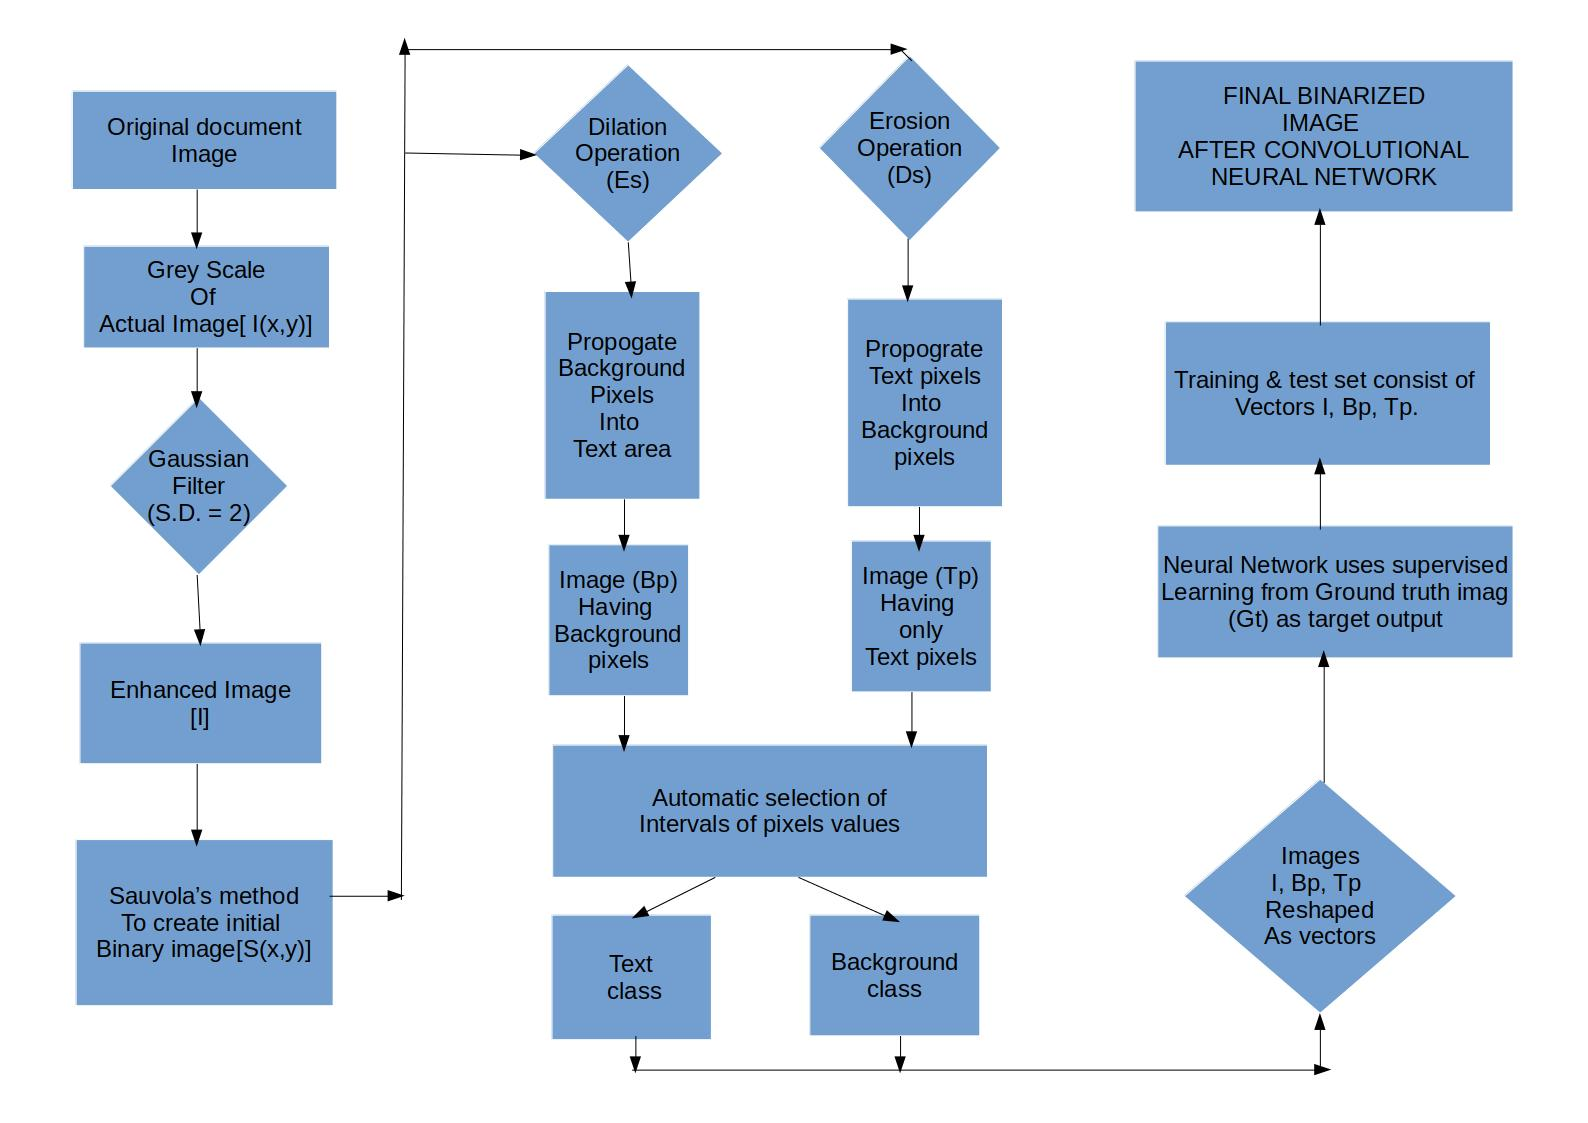
\includegraphics[width=\textwidth]{system_architecture.jpg}
%	\caption{Flow chart for the system}
%\end{figure}
%\subsection{System Feature 1(Functional Requirement)}
%\subsection{System Feature 2(Functional Requirement)}
%\subsection{System Feature n(Functional Requirement)}


\section{External Interface Requirements (If Any)}
\subsection{User Interfaces}
The Graphical User Interface of the proposed system is to be developed using Python Tkinter and PyQt5. \\
The GUI consist of basic button for image input which is to be uploaded in run-time. The output button to show the final output according to different input parameter. These parameters are also taken input from the user.GUI also show what classification is used and the accuracy of the model.
\begin{figure}[!htbp]
    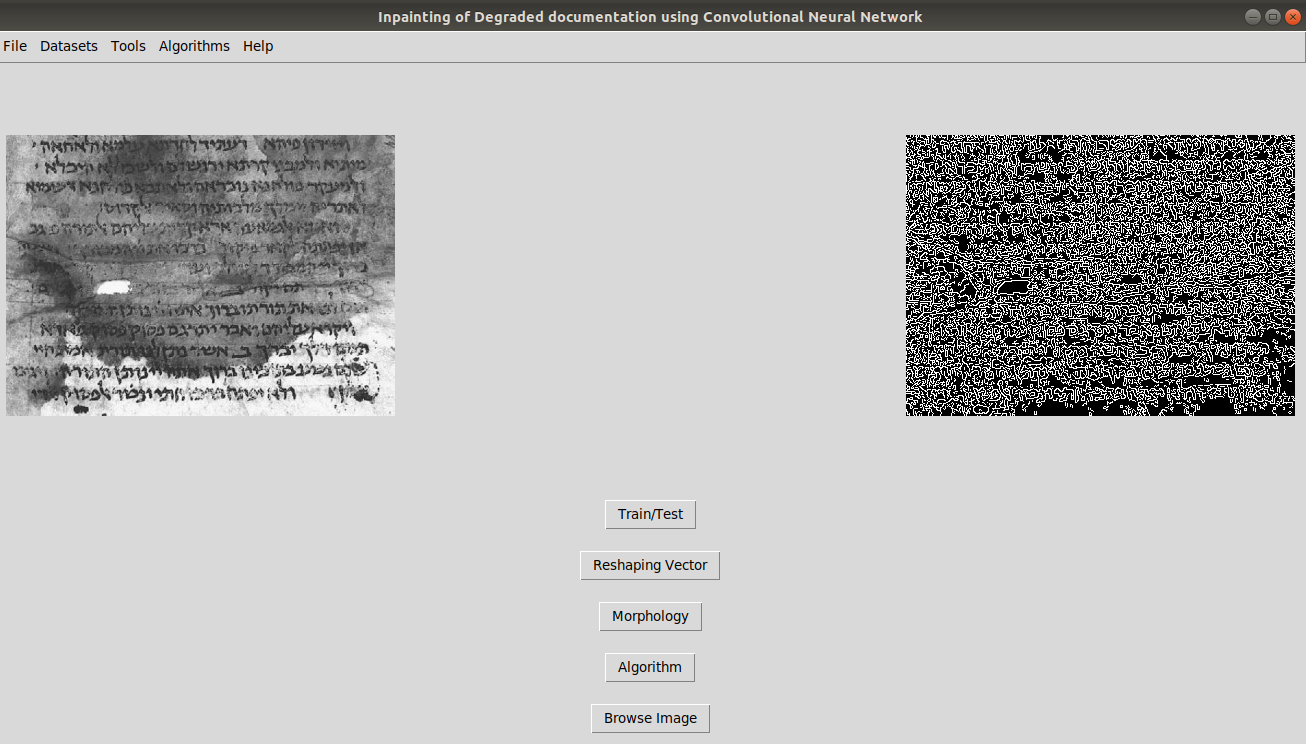
\includegraphics[width=\textwidth]{GUI.png}
	\caption{Graphical User Interface of the system}
\end{figure}
%\subsection{Hardware Interfaces}
\subsection{Software Interfaces}
We have came across a very dynamic and awesome graphical user interfacing tool called \hyperlink{http://www.gnipsel.com/glade/}{Glade} , which uses Gtk3+ and python3 to compatible with.

%\subsection{Communication Interfaces}

\section{Non Functional Requirements}
GUI will be our interface Requirements : Proper classification and training will provide proper output. \\
Requirements : As our system is fully software oriented we don’t need any safety requirement.
\subsection{Performance Requirements}
Since our system is dealing with images and lots of high performance algorithm to work on we will be using Graphics Cards to enhance the system performance and to run the system without any glitch. NVIDIA Graphics card is recommended as they are fast and more reliable when it comes to deep learning.
%\subsection{Safety Requirements}
%\subsection{Security Requirements}
%\subsection{Software Quality Attributes}

\section{System Requirements}
These requirements are used by our team for the system to run efficiently:
\begin{itemize}
    \item Architecture:        x86\_64
    \item Model name:          Intel(R) Core(TM) i5-4210U CPU @ 1.70GHz
    \item Operating System:    Ubuntu 16.04 \& above
    \item Memory(RAM):         4-Gigabits
    \item Graphics Card:       2-Gigabits
    \item Language:            Python version 3.5 \& above.
    \item Python Tools:        Tkinter, PyQt5, Scipy, Scikit-learn, scikit-image, tensorflow, OpenCV2.
\end{itemize}
\subsection{Data sets Requirements}
\begin{itemize}
    \item We will be implementing our project on DIBCO-2009 and DIBCO-2010 data set which is available.\\
\url{http://users.iit.demokritos.gr/~bgat/DIBCO2009/}\\
\url{http://users.iit.demokritos.gr/~bgat/H-DIBCO2010/}

\item LRDE Document Binarization Dataset\\
\url{https://www.lrde.epita.fr/wiki/Olena/DatasetDBD}

\end{itemize}

\subsection{Software Requirements (Platform Choice)}
Our project is entirely implemented and tested on Ubuntu 18.04 LTS.
%\subsection{Hardware Requirements}

\section{Analysis Models : SDLC Model applied}
Agile Software Development Life Cycle models is implemented on the development of the project.In the agile methodology after every development iteration, the customer is able to see the result and understand if he is satisfied with it or he is not. This is one of the advantages of the agile software development life cycle model. One of its disadvantages is that with the absence of defined requirements it is difficult to estimate the resources and development cost.\\
\begin{figure}[!htbp]
    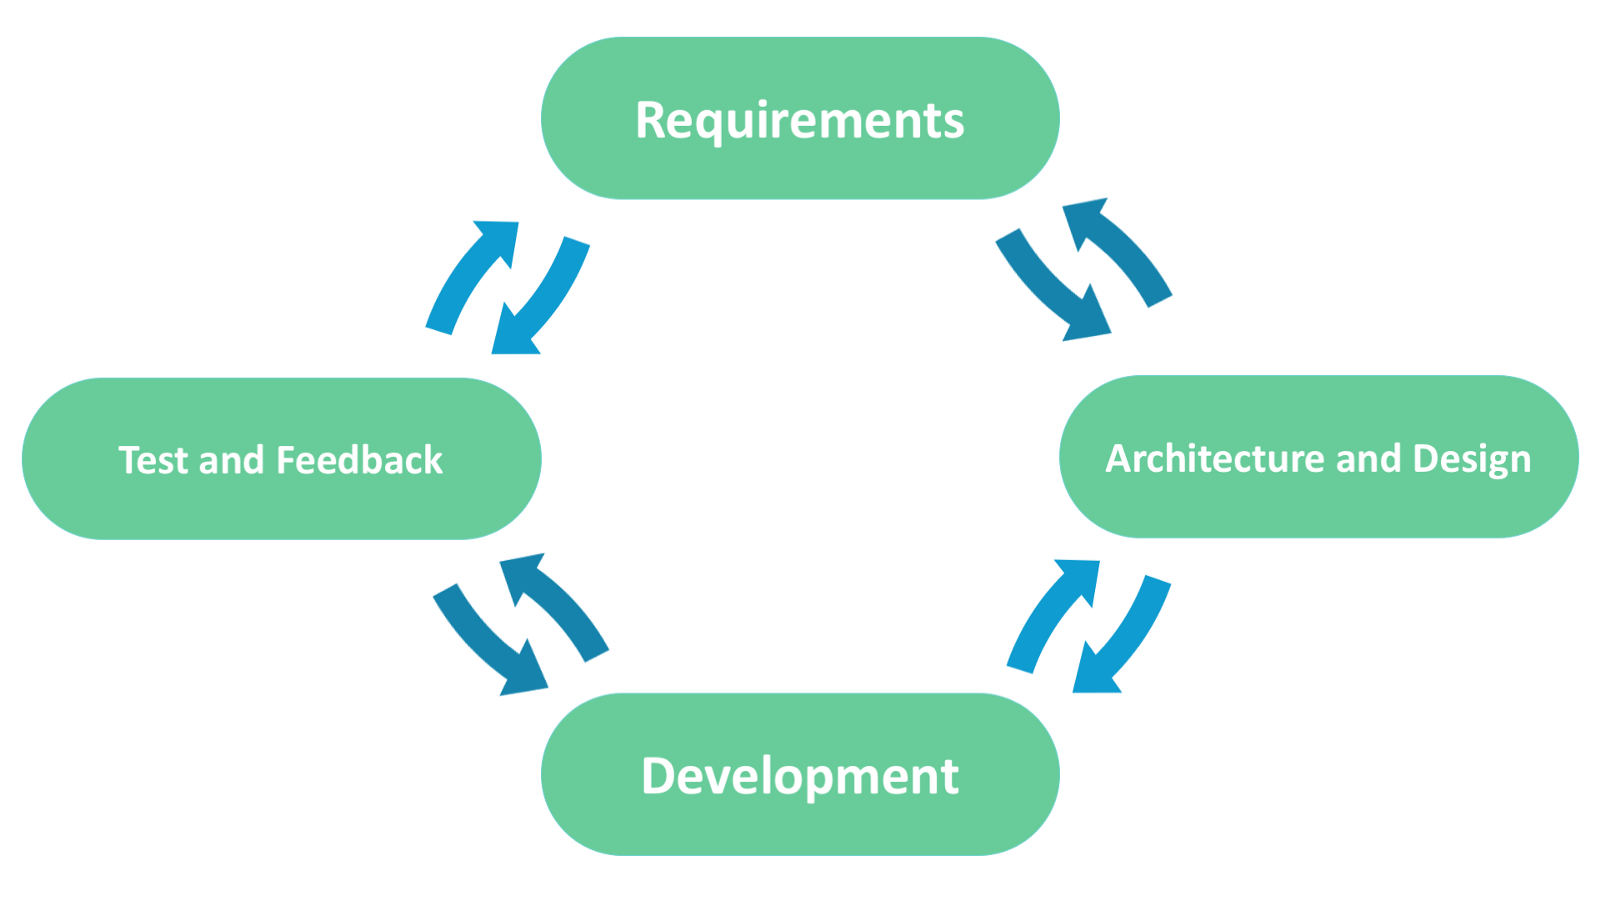
\includegraphics[width=\textwidth]{SDLC.png}
	\caption{Software Development Life Cycle}
\end{figure}







\chapter{System Design}
\section{System Architecture}
\begin{figure}[!htbp]
    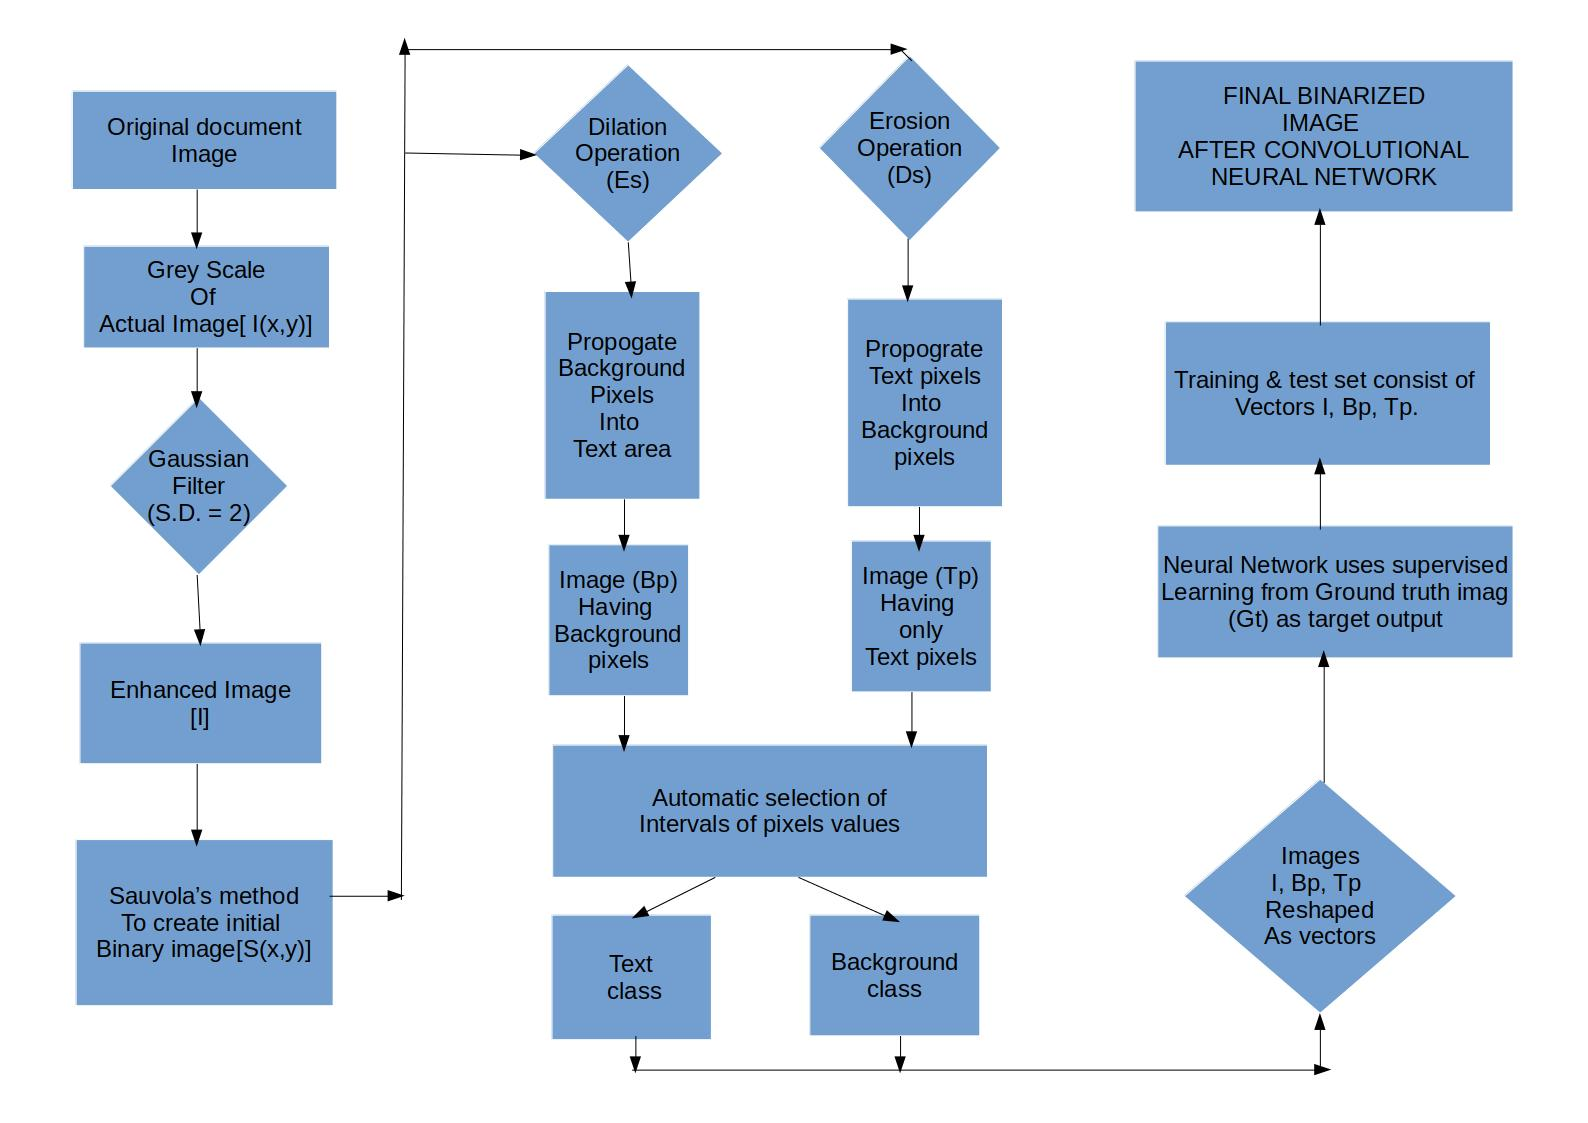
\includegraphics[width=\textwidth]{system_architecture.jpg}
	\caption{Flow chart for the system}
\end{figure}
\section{Mathematical Model}
Without a solid understanding of deep learning, we can only have a set of empirical rules and intuitions, which is not sufficient to advance the scientific knowledge profoundly. There has been a large amount of efforts devoted to the understanding of CNNs from various angles.
In the CNN training, weights are first initialized and then adjusted by back-propagation to minimize a cost function.
Each convolutional layer is specified by its filter weights which are determined in the training stage by an iterative update process. That is, they are first initialized and then adjusted by backpropagation to minimize a cost function. All weights are then fixed in the testing stage. These weights play the role of “system memory”. In this work, we adopt a different name for filter weights to emphasize their role in the testing stage. We call them “anchor vectors” since they serve as reference signals (or visual patterns) for each input patch of test images. It is well-known that signal convolution can also be viewed as signal correlation or projection. For an input image patch, we compute its correlation with each anchor vector to measure their similarity. Clearly, the projection onto a set of anchor vectors offers a spectral decomposition of an input.\\
We define two anchor matrices:\\
          A = [a1, ¨ ¨ ¨ , ak ¨ ¨ ¨ , aK],\\
          B = [b1, ¨ ¨ ¨ , bl ¨ ¨ ¨ , bL] 
\\ Clearly, A ∈ Rˆn×k and B ∈ Rˆk×l .
For the correlation part, let y = AˆT x and z = BˆT y. Then, we have z = B ˆT AˆT x = C ˆT x, C ≡ AB.
Mathematically, we can decompose final CNN output:\\
 x = ∑ (N n=1) x(n)e(n)   
 
\section{Data Flow Diagram}
%\subsection{Different Phases of the System}
\begin{figure}[!htbp]
    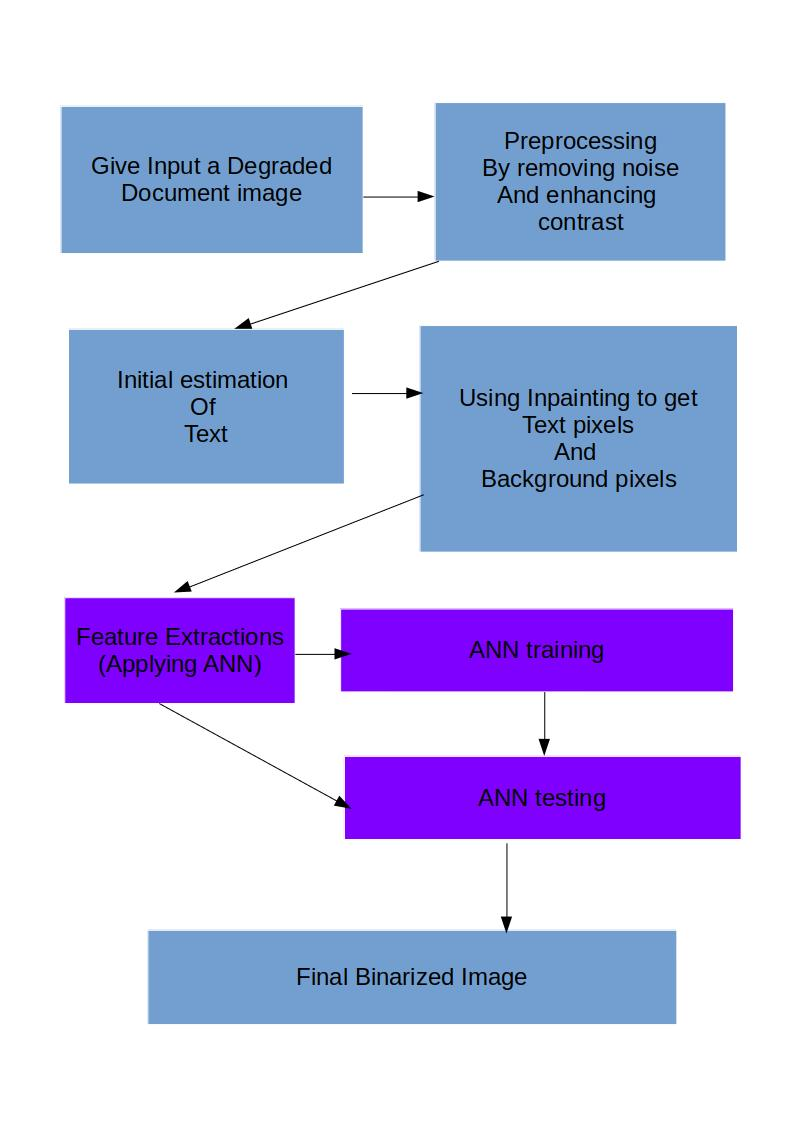
\includegraphics[width=\textwidth]{phases.jpg}
	\caption{Flow chart for the system}
\end{figure}

%\section{Entity Relationship Diagram}
\section{UML Diagram}
The following diagrams show the basic working of the neural network of any deep learning project.\\
\begin{figure}
    \centering
    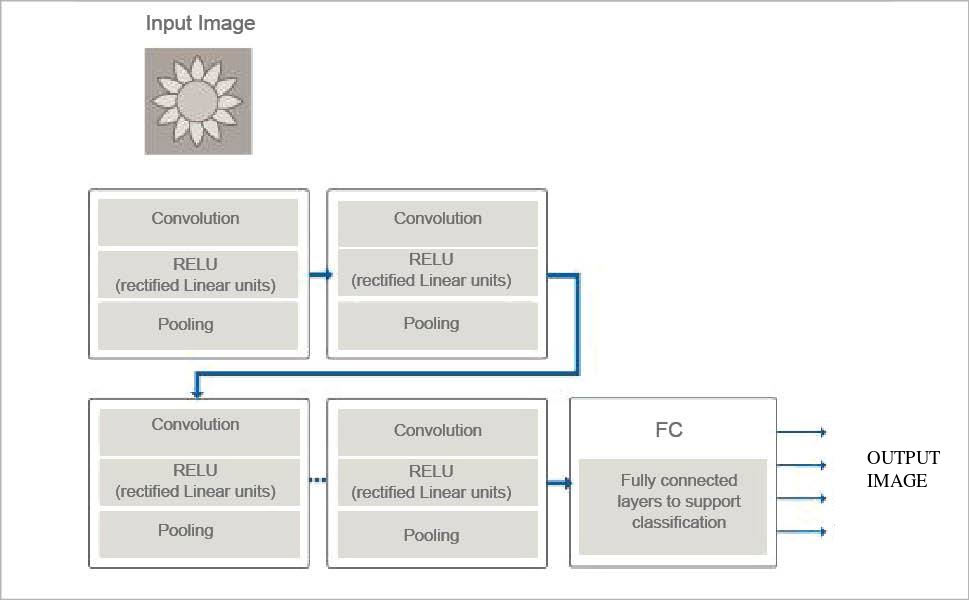
\includegraphics[width=\textwidth]{Neural-network-data-training-approach.png}
    \caption{Basic Neural Network }
    \label{fig:my_label}
\end{figure}
\\
The second diagram represent the flow of the fully loaded neural network.
\begin{figure}
    \centering
    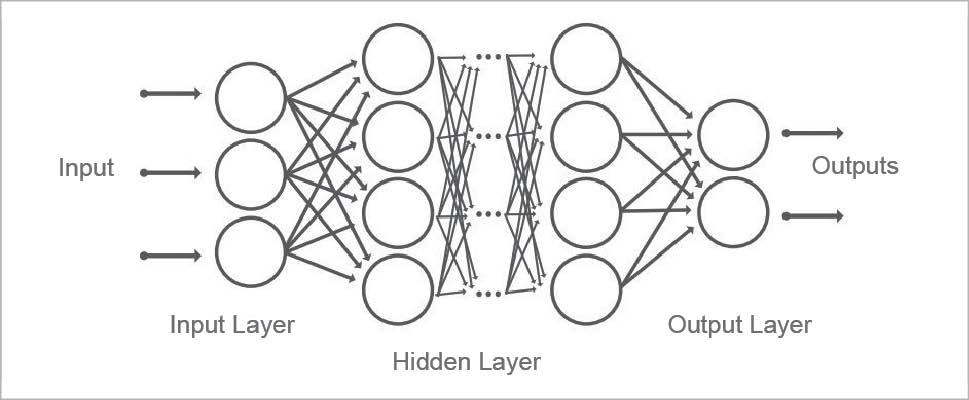
\includegraphics[width=\textwidth]{Deep-learning-neural-networks.jpg}
    \caption{Fully loaded Neural Network}
    \label{fig:my_label}
\end{figure}

\chapter{Project Plan}

\section{Project Estimate}
\subsection{Reconciled Estimate}
\subsection{Project Resources}

\section{Risk Management}
\subsection{Risk Identification}
\subsection{Risk Analysis}
\subsection{Overview of Risk Mitigation, Monitoring, Management}


\section{Project Schedule}
\subsection{Project Task Set}
\subsection{Task Network}
\subsection{Timeline Chart}

\section{Team Organization}
\subsection{Team Structure}
\subsection{Management Reporting and Communication}

\chapter{Project Implementation }

\section{Overview of Project Modules}
This project consists of total five modules. First module works mainly on the input of image to the system and converting that image to Gray-scale and applying Gaussian Filter to produce enhanced image(I). Second module takes enhanced image(I) as input to the respective algorithm we want to apply, which produces a resulting image [S(x,y)]. Third module focuses on Morphology technique i.e. applying dilation operation and erosion operation simultaneously. Dilation operation propagate text pixels into background pixels giving us text pixels(Tp) where as erosion operation propagate the background pixels into text area giving us background pixels(Bp). Fourth module is created so that the model can automatically make selection of intervals of pixel values resulting in Text class and Background class respectively. Then these pixels are reshaped vectors which are used for features selection and feature validation of the images. Final module will do the task of splitting the data-set into training and testing data-sets. Our model is trained using training data-set and learns from available features. This module also display the output image of the system along with necessary output which help us in understanding the model such as: Ground Truth, Accuracy, etc.

\section{Tools and Technology used}
Various tools are used while developing this project. Our whole project is developed in Python3.5+ and various python modules like Scikit-learn, Scikit-image, Numpy, Scipy, Matplotlib, OpenCV3.\\
Graphical User interface is also developed in python GUI framework Tkinter and Glade.\\
Deep Learning tools such as Keras having Tensorflow in backend.
\section{Algorithm Details}
We have give option to the user that which algorithm they want to perform on the input image.
\subsection{Otsu's Algorithm}
Otsu's method is used to automatically perform clustering-based image thresholding, or, the reduction of a graylevel image to a binary image.The algorithm assumes that the image contains two classes of pixels following bi-modal histogram (foreground pixels and background pixels), it then calculates the optimum threshold separating the two classes so that their combined spread (intra-class variance) is minimal, or equivalently (because the sum of pairwise squared distances is constant), so that their inter-class variance is maximal.\\
Algorithm:\\
\begin{itemize}
    \item Compute histogram and probabilities of each intensity level
    \item Set up initial {\displaystyle \textomega _{i}(0)} \textomega \textunderscore{i}(0) and {\displaystyle \textmu \textunderscore{i}(0)} \textmu \textunderscore{i}(0)
    \item Step through all possible thresholds {\displaystyle t=1,\ldots } {\displaystyle t=1,\ldots } maximum intensity
    \begin{itemize}
        \item Update {\displaystyle \textomega \textunderscore{i}} \textomega \textunderscore{i} and {\displaystyle \textmu \textunderscore{i}} \textmu \textunderscore{i}
        \item Compute {\displaystyle \textsigma \textunderscore{b}^{2}(t)} \textsigma \textunderscore{b}^{2}(t)
    \end{itemize}
\end{itemize}
\subsection{Algorithm 2}
\subsection{Algorithm n}


\chapter{Software Testing }
\section{Types of Testing}
\section{Test Cases and Test Results}

\chapter{Results}
\section{Outcomes}
\section{Screen Shots}


\chapter{Conclusions}
\section{Conclusion}
\section{Future Work}
\section{Applications}




\begin{appendices}


% \chapter{ALGORITHMIC DESIGN}
\chapter{}
Problem statement feasibility assessment using, satisfiability analysis and NP Hard, NP-Complete or P type using modern algebra and relevant mathematical models








\chapter{ }
Details of paper publications: name of the conference/journal, comments of reviewers, certificate, paper. 

\chapter{Plagiarism Report}
Plagiarism report of project report


\chapter{References}
Thomas Noltey, Hans Hanssony, Lucia Lo Belloz,”Communication Buses for Automotive Applications” In Proceedings of the 3rd Information Survivability Workshop (ISW-2007), Boston, Massachusetts, USA, October 2007. IEEE Computer Society.

\end{appendices}


\end{document}
